\begin{table}[H]
\centering
\caption{Sample construction and selection diagnostics}
\label{tab:sample_selection}
\begin{tabular}{lcccc}
\toprule
 & \multicolumn{2}{c}{Households} & Observations &  \\
\cmidrule(lr){2-3}
Step & Control & Information & Total & p-value \\
\midrule

Initial sample 
& 506 & 514 & 11,085,928 &  \\

Remove PV households 
& 454 & 457 & 9,872,084 & 0.67 \\

Coverage $>$ 90\% 
& 453 & 453 & 9,829,654 & 0.22 \\

Remove bad days 
& 453 & 453 & 9,791,350 & 0.99 \\

Remove outliers (3 SD rule) 
& 443 & 449 & 9,636,515 & 0.43 \\

Balanced pre-treatment window 
& 443 & 449 & 8,495,920 &  \\

\midrule
Final sample 
& 443 & 449 & 8,495,920 &  \\

\bottomrule
\end{tabular}

\caption*{\footnotesize
Note: This table documents the sequential construction of the estimation sample. The first columns report the number of households in the control and information groups after each step. The observation column reports the total number of hourly observations. The final column shows p-values from logistic regressions of a removal indicator on treatment status, testing for differential attrition. We find no systematic evidence of differential attrition across groups.}
\end{table}

\begin{sidewaystable}[p]
\centering
\caption{Monthly App Engagement by Tranche}
\label{tab:monthly_engagement_landscape}
\scriptsize
\setlength{\tabcolsep}{3pt}

\begin{tabular*}{\textheight}{@{\extracolsep{\fill}} l ccc | ccc | ccc}
\toprule
& \multicolumn{3}{c}{\textbf{Tranche 1 (N = 171)}} 
& \multicolumn{3}{c}{\textbf{Tranche 2 (N = 196)}} 
& \multicolumn{3}{c}{\textbf{Tranche 3 (N = 82)}} \\
\cmidrule(lr){2-4} \cmidrule(lr){5-7} \cmidrule(lr){8-10}

Month 
& Active (\%) & Mean & Total
& Active (\%) & Mean & Total
& Active (\%) & Mean & Total \\

\midrule

0  & 124 (73) & 25.5 & 3160 & 102 (52) & 15.5 & 1585 & 46 (56) & 12.8 & 588 \\
1  &  64 (37) & 20.4 & 1307 &  69 (35) & 24.5 & 1690 & 31 (38) & 27.2 & 842 \\
2  &  36 (21) & 28.1 & 1013 &  47 (24) & 26.1 & 1225 & 19 (23) & 35.5 & 674 \\
3  &  24 (14) & 26.1 &  627 &  34 (17) & 28.9 &  982 & 17 (21) & 34.1 & 580 \\
4  &  28 (16) & 20.9 &  586 &  33 (17) & 27.7 &  915 & 15 (18) & 29.9 & 448 \\
5  &  23 (14) & 24.4 &  560 &  30 (15) & 26.4 &  793 & 12 (15) & 29.8 & 358 \\
6  &  19 (11) & 29.4 &  559 &  32 (16) & 28.6 &  914 & 14 (17) & 19.8 & 277 \\
7  &  20 (12) & 31.6 &  631 &  26 (13) & 28.2 &  733 & 13 (16) & 24.4 & 317 \\
8  &  17 (10) & 27.8 &  473 &  33 (17) & 19.8 &  653 &  8 (10) & 44.0 & 352 \\
9  &  17 (10) & 34.0 &  578 &  25 (13) & 28.4 &  710 & 11 (13) & 28.0 & 308 \\
10 &  14 (8)  & 32.1 &  449 &  18 (9)  & 29.7 &  534 & 11 (13) & 29.0 & 319 \\
11 &  20 (12) & 24.7 &  494 &  19 (10) & 33.3 &  633 & 13 (16) & 18.3 & 238 \\
12 &  14 (8)  & 34.4 &  482 &  20 (10) & 18.1 &  361 & --      & --   & --  \\
13 &  10 (6)  & 44.0 &  440 &  31 (16) &  8.8 &  272 & --      & --   & --  \\
14 &  11 (6)  & 39.6 &  436 & --       & --   & --   & --      & --   & --  \\
15 &  14 (8)  & 28.8 &  403 & --       & --   & --   & --      & --   & --  \\
16 &  23 (14) & 10.5 &  242 & --       & --   & --   & --      & --   & --  \\

\bottomrule
\end{tabular*}

\caption*{\scriptsize
\textit{Note:} ``Active (\%)'' reports the number and share of households with at least one interaction in a given month since treatment. Mean denotes the average number of interactions among active users. Total reports the total number of interactions per month. Later months are not observed for all tranches due to the staggered rollout of the intervention.}
\end{sidewaystable}


\begin{table}[htbp]
\centering
\caption{Comparison of Sample Households with Upper Austria and Austria}
\label{tab:sample_comparison}
\begin{threeparttable}
\begin{tabular}{lccc}
\toprule
 & Sample & Upper Austria & Austria \\
\midrule
Apartment (share)              & 0.280 & 0.610 & 0.460 \\
Ownership (share)              & 0.760 & 0.520 & 0.490 \\
Living space (m\textsuperscript{2}) & 133.4 & 107.8 & 99.9 \\
Household size (persons)       & 2.70  & 2.28  & 2.20 \\
Heat pump for heating (share)  & 0.310 & 0.110 & 0.100 \\
Electric car (share)           & 0.015 & 0.004 & 0.004 \\
Dryer (share)                  & 0.570 & 0.450 & 0.410 \\
Computer (share)               & 0.980 & 0.720 & 0.730 \\
\bottomrule
\end{tabular}
\begin{tablenotes}[flushleft]
\footnotesize
\item Population figures refer to households in Upper Austria and Austria. Sample figures refer to households in the final analysis sample.
\end{tablenotes}
\end{threeparttable}
\end{table}

\begin{figure}
\centering
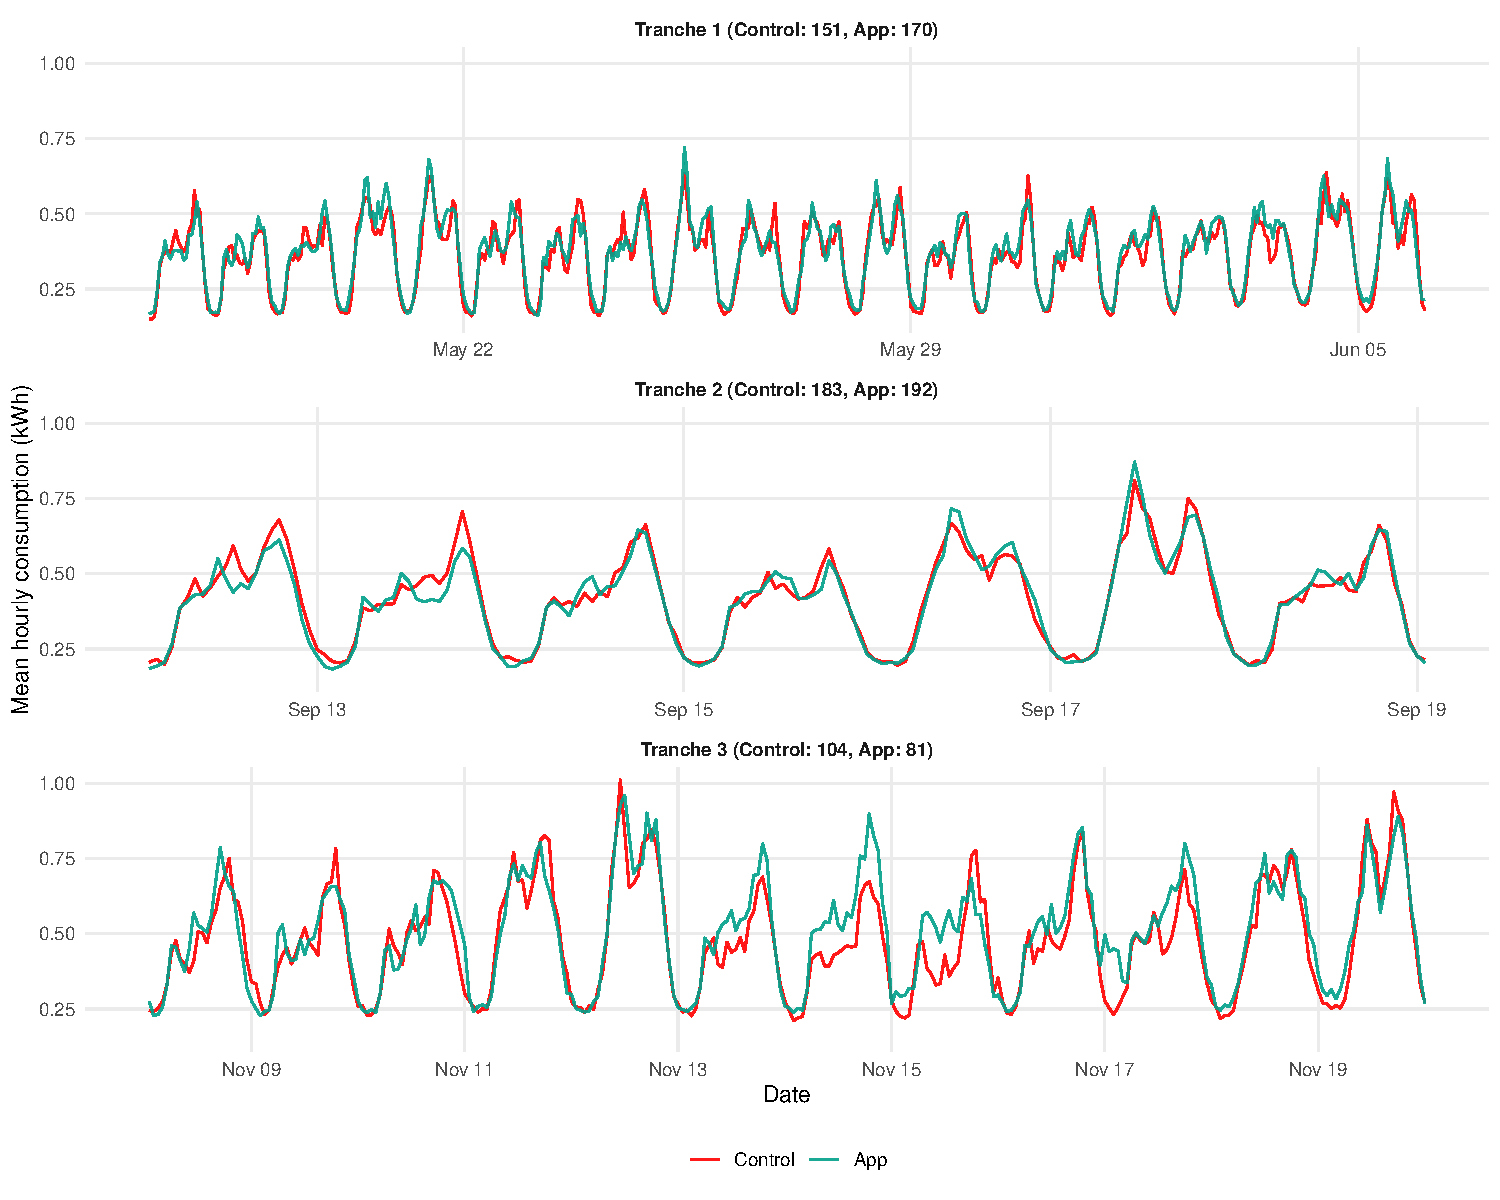
\includegraphics[width=1\linewidth]{paper/figures/descriptive_hourly_pre_by_tranche_calendar.pdf}
\caption{Pre-treatment hourly electricity consumption by tranche and group over time. Panels are shown for each tranche. }
\label{fig:tranche_pre_calendar}
\end{figure}

\begin{table}[htbp]
\centering
\caption{Dynamic Treatment Effects by Consumption Type}
\label{tab:event_study_full}
\begin{threeparttable}
\scriptsize
\begin{tabular}{lccc lccc}
\toprule
\multicolumn{4}{c}{\textbf{Weeks $-3$ to $24$}} & \multicolumn{4}{c}{\textbf{Weeks $25$ to $50+$}} \\
\cmidrule(lr){1-4} \cmidrule(lr){5-8}
 & Total & Daytime & Non-daytime &  & Total & Daytime & Non-daytime \\
\midrule

Week $-3$ & -0.088 & -0.148 & 0.060 & Week $25$ & -0.512 & -0.359 & -0.154 \\
          & (0.313) & (0.261) & (0.078) &           & (0.371) & (0.268) & (0.144) \\

Week $-2$ & -0.245 & -0.276 & 0.029 & Week $26$ & -0.396 & -0.260 & -0.139 \\
          & (0.247) & (0.223) & (0.051) &           & (0.430) & (0.307) & (0.161) \\

Week $0$  & -0.012 & -0.007 & -0.006 & Week $27$ & -0.823** & -0.580** & -0.245 \\
          & (0.135) & (0.111) & (0.044) &           & (0.413)  & (0.292)  & (0.161) \\

Week $1$  & -0.243 & -0.257* & 0.014 & Week $28$ & -0.338 & -0.271 & -0.068 \\
          & (0.158) & (0.136) & (0.045) &           & (0.366) & (0.271) & (0.131) \\

Week $2$  & -0.365** & -0.300** & -0.066 & Week $29$ & -0.644* & -0.532* & -0.113 \\
          & (0.175)  & (0.150)  & (0.052) &           & (0.380)  & (0.281)  & (0.136) \\

Week $3$  & -0.572** & -0.476** & -0.096* & Week $30$ & -0.489 & -0.369 & -0.122 \\
          & (0.184)  & (0.154)  & (0.057) &           & (0.338) & (0.261) & (0.114) \\

Week $4$  & -0.428** & -0.365** & -0.065 & Week $31$ & -0.272 & -0.140 & -0.133 \\
          & (0.185)  & (0.154)  & (0.059) &           & (0.318) & (0.233) & (0.125) \\

Week $5$  & -0.637** & -0.536** & -0.102* & Week $32$ & -0.488 & -0.290 & -0.199 \\
          & (0.216)  & (0.179)  & (0.062) &           & (0.396) & (0.286) & (0.147) \\

Week $6$  & -0.361 & -0.271 & -0.092 & Week $33$ & -0.327 & -0.159 & -0.170 \\
          & (0.242) & (0.191) & (0.072) &           & (0.370) & (0.273) & (0.132) \\

Week $7$  & -0.344 & -0.326* & -0.021 & Week $34$ & -0.366 & -0.195 & -0.172 \\
          & (0.206) & (0.169) & (0.069) &           & (0.326) & (0.239) & (0.132) \\

Week $8$  & -0.447* & -0.418** & -0.029 & Week $35$ & -0.534 & -0.325 & -0.211 \\
          & (0.232) & (0.183) & (0.085) &           & (0.343) & (0.249) & (0.135) \\

Week $9$  & -0.611** & -0.525** & -0.087 & Week $36$ & -0.412 & -0.228 & -0.184 \\
          & (0.271)  & (0.204)  & (0.101) &           & (0.332) & (0.246) & (0.135) \\

Week $10$ & -0.817** & -0.638** & -0.180* & Week $37$ & -0.451 & -0.220 & -0.232* \\
          & (0.300)  & (0.227)  & (0.102) &           & (0.328) & (0.247) & (0.128) \\

Week $11$ & -0.978** & -0.759** & -0.218* & Week $38$ & -0.608* & -0.347 & -0.262* \\
          & (0.324)  & (0.236)  & (0.119) &           & (0.330) & (0.244) & (0.137) \\

Week $12$ & -0.410 & -0.321 & -0.087 & Week $39$ & -0.279 & -0.105 & -0.168 \\
          & (0.438) & (0.309) & (0.151) &           & (0.300) & (0.228) & (0.118) \\

Week $13$ & -0.631 & -0.527* & -0.105 & Week $40$ & -0.195 & -0.107 & -0.091 \\
          & (0.418) & (0.300) & (0.141) &           & (0.293) & (0.227) & (0.116) \\

Week $14$ & -0.293 & -0.209 & -0.092 & Week $41$ & -0.200 & -0.109 & -0.096 \\
          & (0.425) & (0.291) & (0.160) &           & (0.305) & (0.228) & (0.121) \\

Week $15$ & -0.407 & -0.315 & -0.093 & Week $42$ & -0.353 & -0.208 & -0.148 \\
          & (0.313) & (0.226) & (0.122) &           & (0.305) & (0.234) & (0.117) \\

Week $16$ & -0.477* & -0.370* & -0.108 & Week $43$ & -0.262 & -0.149 & -0.115 \\
          & (0.271) & (0.201) & (0.107) &           & (0.268) & (0.215) & (0.096) \\

Week $17$ & -0.756** & -0.548** & -0.209 & Week $44$ & -0.162 & -0.085 & -0.078 \\
          & (0.384)  & (0.272)  & (0.142) &           & (0.274) & (0.219) & (0.097) \\

Week $18$ & -0.629* & -0.461* & -0.170 & Week $45$ & -0.303 & -0.207 & -0.098 \\
          & (0.366) & (0.264) & (0.131) &           & (0.288) & (0.228) & (0.099) \\

Week $19$ & -0.420 & -0.301 & -0.119 & Week $46$ & -0.390 & -0.247 & -0.144 \\
          & (0.301) & (0.224) & (0.115) &           & (0.291) & (0.221) & (0.117) \\

Week $20$ & -0.546 & -0.423* & -0.123 & Week $47$ & -0.266 & -0.153 & -0.114 \\
          & (0.332) & (0.248) & (0.121) &           & (0.285) & (0.212) & (0.128) \\

Week $21$ & -0.497 & -0.368 & -0.131 & Week $48$ & -0.300 & -0.159 & -0.143 \\
          & (0.341) & (0.249) & (0.135) &           & (0.291) & (0.224) & (0.108) \\

Week $22$ & -0.777** & -0.578** & -0.199 & Week $49$ & -0.467 & -0.289 & -0.179 \\
          & (0.363)  & (0.265)  & (0.139) &           & (0.291) & (0.215) & (0.119) \\

Week $23$ & -0.802* & -0.579* & -0.221 & Week $50$ & -0.396 & -0.190 & -0.208* \\
          & (0.426) & (0.298) & (0.169) &           & (0.299) & (0.220) & (0.123) \\

Week $24$ & -0.709** & -0.537** & -0.172 & Week $50+$ & -0.550 & -0.330 & -0.230 \\
          & (0.341)  & (0.248)  & (0.131) &            & (0.430) & (0.320) & (0.170) \\

\bottomrule
\end{tabular}
\begin{tablenotes}[flushleft]
\footnotesize
\item The table reports dynamic treatment effects relative to the week prior to treatment. Standard errors clustered at the household level are reported in parentheses. Week $50+$ reports the average effect for all weeks beyond week 50. Significance levels: ** $p<0.05$, * $p<0.10$.
\end{tablenotes}
\end{threeparttable}
\end{table}



\begin{table}[htbp]
\centering
\caption{Pre-Treatment Electricity Consumption (kWh/day) by Engagement Group}
\label{tab:pre_engagement}
\begin{threeparttable}
\begin{tabular}{lcccc}
\toprule
 & Baseline & High & Medium & Low \\
\midrule
\textbf{Panel A: Tranche 1 (20 pre-days)} \\
Mean (SE) & 8.639 & 8.564 & 8.703 & 9.464 \\
 & (0.095) & (0.212) & (0.193) & (0.202) \\
Diff. vs Baseline & -- & $-0.075$ & $0.064$ & $0.825$ \\
HHs & 192 & 35 & 49 & 45 \\
\midrule
\textbf{Panel B: Tranche 2 (7 pre-days)} \\
Mean (SE) & 9.419 & 9.701 & 11.673 & 8.236 \\
 & (0.158) & (0.384) & (0.365) & (0.360) \\
Diff. vs Baseline & -- & $0.282$ & $2.254$ & $-1.183$ \\
HHs & 261 & 38 & 37 & 39 \\
\midrule
\textbf{Panel C: Tranche 3 (12 pre-days)} \\
Mean (SE) & 10.829 & 13.746 & 10.795 & 10.963 \\
 & (0.193) & (0.682) & (0.540) & (0.690) \\
Diff. vs Baseline & -- & $2.917$ & $-0.034$ & $0.134$ \\
HHs & 136 & 18 & 12 & 19 \\
\midrule
\multicolumn{5}{l}{\textit{Standard errors clustered at household level. Differences unadjusted.}} \\
\bottomrule
\end{tabular}
\begin{tablenotes}[flushleft]
\footnotesize
\item Baseline = Control + Never-engaged app households. Engagement categories from post-treatment login tertiles. Pre-treatment means weighted by available days per tranche. Patterns are descriptive; post-treatment engagement measurement may correlate with unobserved baseline characteristics. Household counts sum to 881 rather than the full analysis sample of 892: 11 households (concentrated in Tranche 2, which has only a 7-day pre-treatment window) have no pre-treatment observations and are therefore excluded from this table.
\end{tablenotes}
\end{threeparttable}
\end{table}
